\documentclass[11pt,a4paper,notitlepage,onecolumn]{article}
\usepackage[german]{babel}
\usepackage[utf8]{inputenc}
\usepackage{graphicx}
\title{Aufgabe2\_3}
\author{Robin Nehls, Yves Müller\\
  Freie Universit\"at Berlin\\
  nehls@spline.de uves@spline.de }
\date{}
\begin{document}

\maketitle

\paragraph{Interpolation}
The first graph that our approximation of the function is in the actually interval 
very close to sqrt(x).

\begin{figure}
\centering
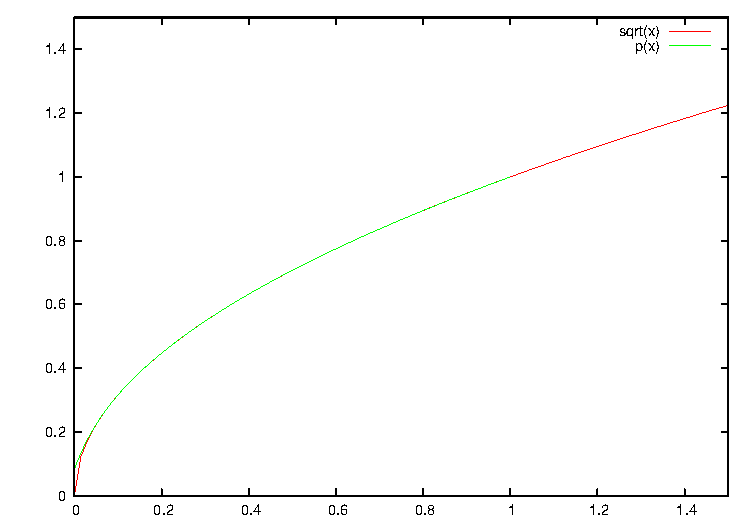
\includegraphics[width=\textwidth]{data/aufgabe4-1IP.pdf}
\caption{\em \small plot of the hole interval using 15 interpolation values}
\end{figure}

\paragraph{Extrapolation}
It is no suprise that the absoulte error becomes bigger as we move away from X1,
also because auf the special charateritcs of the square root function. Using more
interpolation value reduces the absolute error, but in relation to the original
sqrt() the errro remains quite big.

\begin{figure}
\centering
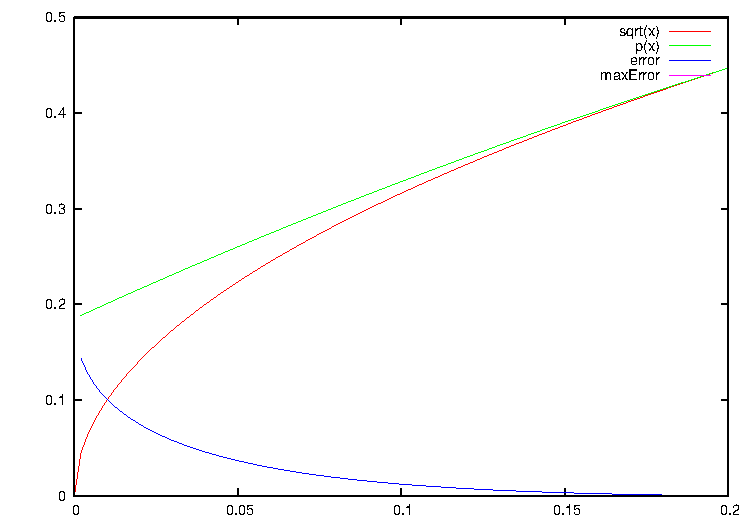
\includegraphics[width=\textwidth]{data/aufgabe4-1based5.pdf}
\caption{\em \small Results using 5 interpolation values}
\end{figure}

\begin{figure}
\centering
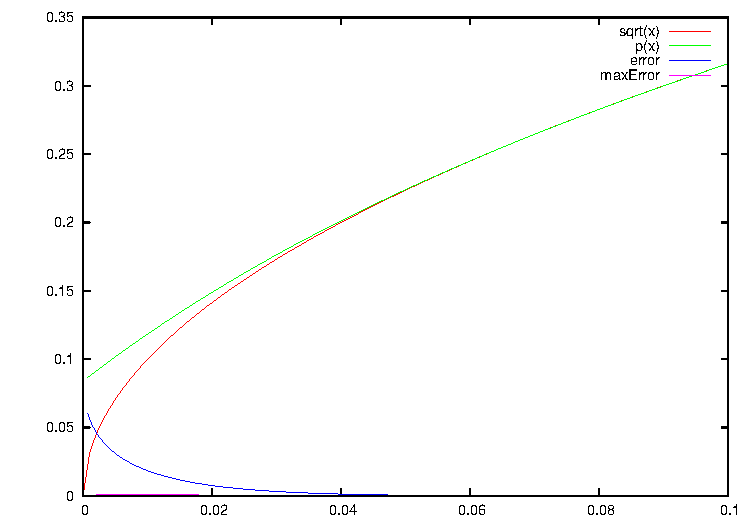
\includegraphics[width=\textwidth]{data/aufgabe4-1based10.pdf}
\caption{\em \small Results using 10 interpolation values}
\end{figure}

\begin{figure}
\centering
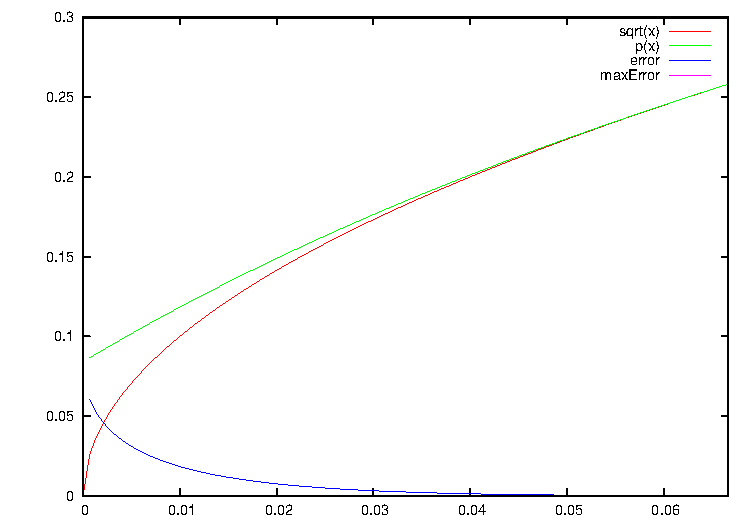
\includegraphics[width=\textwidth]{data/aufgabe4-1based15.pdf}
\caption{\em \small Results using 15 interpolation values}
\end{figure}


\paragraph{Errorcomputation} We modified the formular as follows to compute 
the maximal error. \\ \\
$\Leftrightarrow \frac{f^{(n+1)}(\xi)}{(n+1)!} $ \\ \\
$\Leftrightarrow \frac{\frac{1}{2}(-\frac{1}{2})...(-\frac{2(n+1)-1}{2})}{(n+1)!} $ \\ \\
$\Leftrightarrow \frac{\prod_{i=1}^{n+1}(-\frac{2(i+1)-1}{2})}{\prod_{i=1}^{n+1}i} $ \\ \\
$\Leftrightarrow (-1)^{(n+1)} \prod_{i=1}^{n+1}(1-\frac{3}{2i})$

\paragraph{}
It seems that our code doesen't work so well, when computing the maximum error, 
since the maximal error is way much smaller than our actuall error. This behaviour 
could be caused by extrapolation, but also near the interpolation intervall the
absolute error stays bigger.


\end{document}
